\documentclass[8pt,a4paper]{article}
\usepackage[margin=0.8in]{geometry}
\usepackage[utf8]{inputenc}
\usepackage{amsmath}
\usepackage{amsfonts}
\usepackage{amssymb}
\usepackage[hidelinks]{hyperref}
\usepackage{float}

%s comments
\usepackage{verbatim}

%inline graphs
\usepackage{wrapfig}
% multiple figures on line
\usepackage{subfig}

\usepackage{graphicx}
\graphicspath{ {img/} }

% Caption font size
% https://tex.stackexchange.com/questions/86120/font-size-of-figure-caption-header
\usepackage[font=scriptsize,labelfont=bf]{caption}

\usepackage{fancyhdr}
\pagestyle{fancy}
\lhead{\rightmark}
\chead{}
\rhead{SOFT354 - Parallel Computing and Distributed Systems}
\lfoot{\thepage}
\cfoot{}
\rfoot{Ben Lancaster 10424877}

\renewcommand{\subsectionmark}[1]{\markright{\thesubsection\ #1}}

\begin{document}

\begin{titlepage}
\begin{center}

\vspace*{3cm}
\Large
\textbf{SOFT354 - Parallel Computing and Distributed Systems}

\vspace{0.4cm}
\large
A comparison of the Discrete Fourier Transform algorithm implemented in CUDA and MPI.

\vspace{4cm}
\textbf{Ben Lancaster}\\
\today

\vspace{4cm}
\textbf{Abstract}\\
\small
My placement as a Firmware Engineer at Spirent, a world leader in GNSS simulators. Coming from a Computer Science I was up to speed on the programming aspect of firmware, however was lacking in experience of electronic lab equipment. Constant exposure to this new area of technology and equipment has greatly improved my knowledge in GNSS and embedded programming and has influenced my future career choices. I was chiefly responsible for writing a new programmable timer, implementing fan-control strategies and power calibration schemes, writing a driver to read in peripheral devices, provisioning a Linux hypervisor, and designing and implement a Linux USB driver.

\end{center}

\end{titlepage}

\renewcommand*\contentsname{Table of Contents}
\tableofcontents

\section{Introduction}
This report discusses the implementation and performance of the Discrete Fourier Transform (DFT) algorithm in CUDA and MPI.

DFT is largely used in digital signal and image processing applications. 

In this report, I will be implementing the DFT to convert signals in the time domain to the frequency domain.


\begin{figure}[H]%
    \centering
    \subfloat[Time domain]{{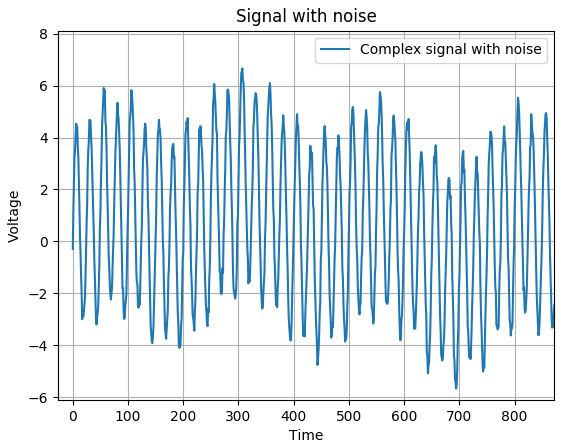
\includegraphics[width=7cm]{intro_signal} }}%
    \qquad
    \subfloat[Frequency domain]{{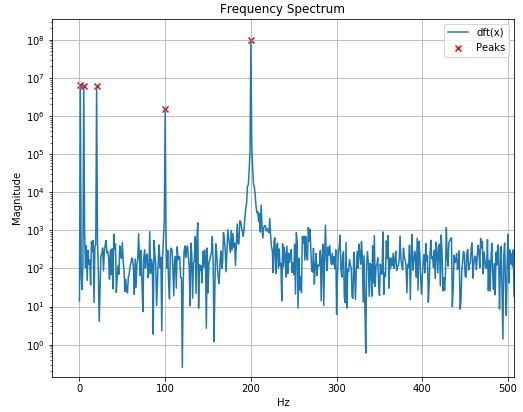
\includegraphics[width=7cm]{intro_dft} }}%
    \vspace{5pt}
    \caption{\textbf{Left:} A compound signal made up of 1, 5, 20, 100, and 200 Hz sine waves in the time domain. \textbf{Right:} Frequency domain representation showing high amplitude peaks for the 1, 5, 20, 100, and 200 Hz waveforms.}%
    \label{fig:gridwatch}%
\end{figure}

\section{Implementation}
\subsection{CUDA}

\subsection{MPI}
With DFT, each sample must have operate on all other samples. In my implementation, I must first copy the complete sample array to each node. 

\begin{figure}[H]
\begin{center}
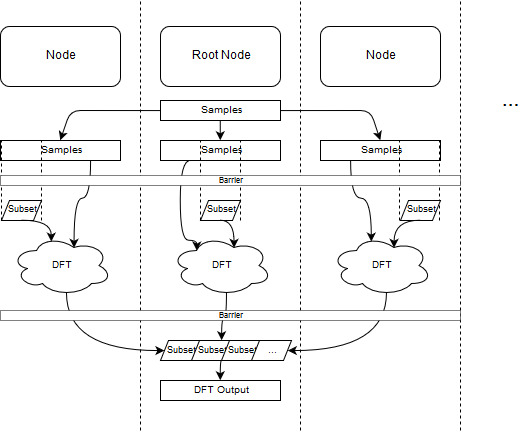
\includegraphics[scale=0.7]{mpi_impl1}
\end{center}
\caption{Control flow diagram for the MPI DFT algorithm.}
\label{fig:train10x}
\end{figure}

\section{Evaluation}
\subsection{Measuring Performance}


\end{document}
